\chapter{実験}\label{chap:test}

\section{実験条件}

実験環境として、図\ref{fig:picture01}を用意する。壁面まで距離1[m]、高さ1[m]地点にカメラを設置する。一面には単色無地のカーテンをかける。なぜカーテンを用いるかという特徴点検出の難しい環境の再現に適しているからである。ORB-SLAM2はFASTキーポイント検出によりエッジから特徴点検出をする。この特徴点を追跡(トラッキング)することでカメラの位置姿勢を推定し、三次元空間における座標計算から環境地図生成をする。このため、エッジの立たない物体であるカーテンから特徴点検出をすることはできずORB-SLAM2が中断される。もう一面には棚を配置する。この棚はエッジが十分に検出可能で、ORB-SLAM2によるトラッキングの開始をスムーズにさせる役割を果たす。

\begin{figure}[h]
        \begin{center}
        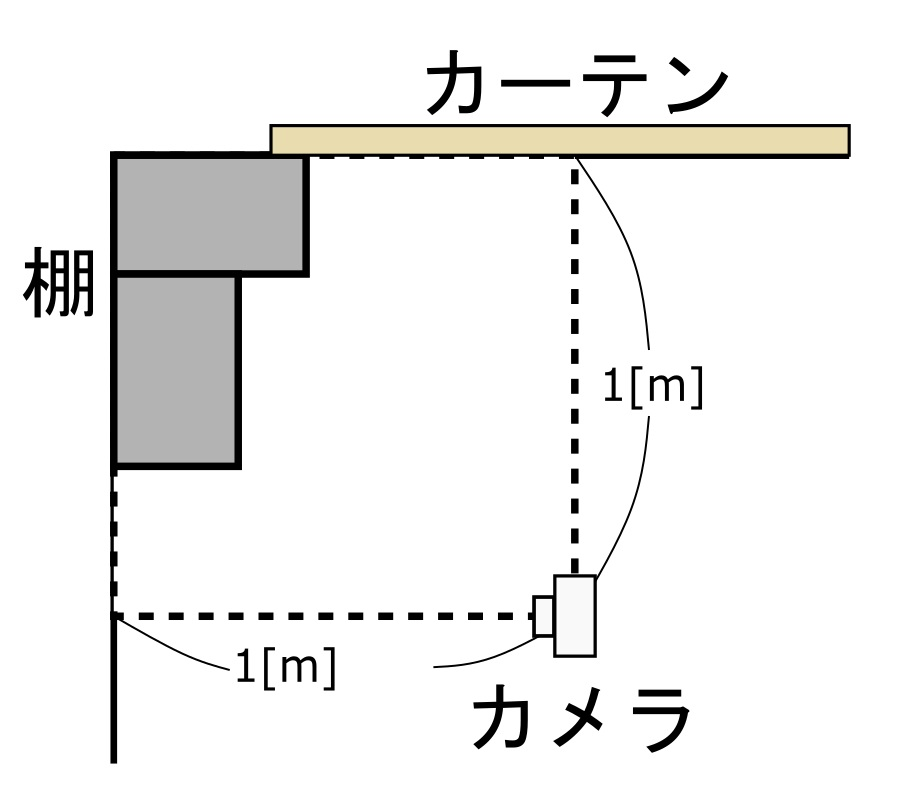
\includegraphics[width=0.7\linewidth]{figs/picture01.jpg}
        \caption{実験環境概略図}
        \label{fig:picture01}
        \end{center}
\end{figure}


\section{実験方法}

ORB-SLAM2を起動し、カメラを棚に向けてトラッキングを開始する。カメラをカーテンへ向けていくとやがて特徴点検出ができなくなり、カメラの画角が図\ref{fig:picture02}赤線部となる位置でトラッキングが停止する。カメラ画像が図\ref{fig:Tracking02}となるこの位置よりカーテン方向へカメラを向けるとトラッキングが停止し、SLAMが中断される。

\begin{figure}[h]
 \begin{tabular}{cc}
      \begin{minipage}[t]{0.45\hsize}
        \centering
        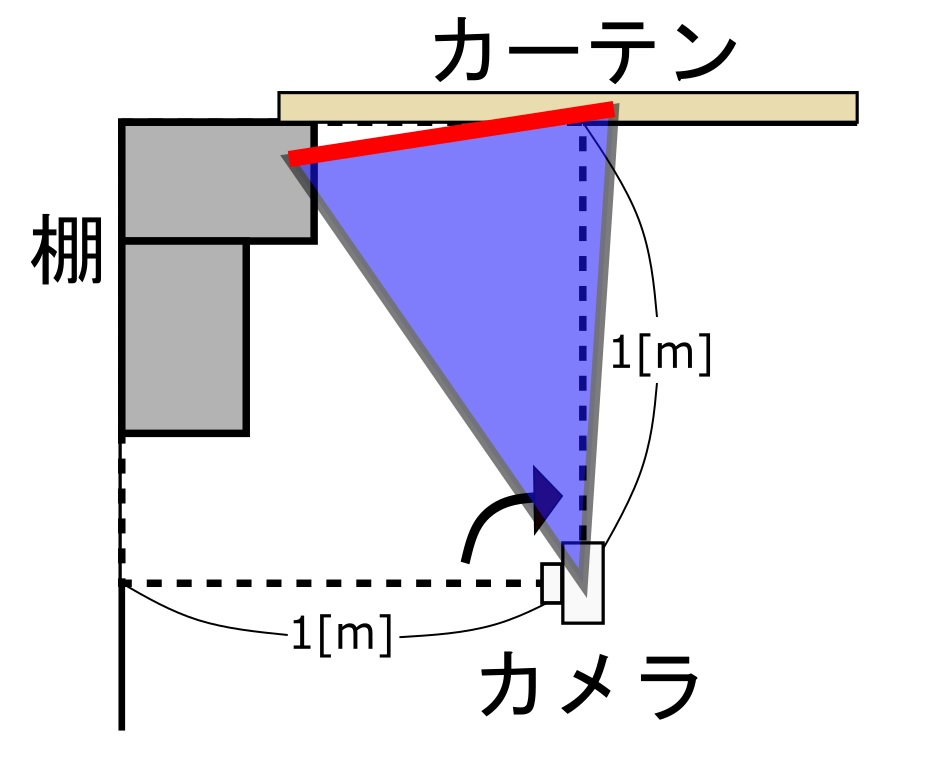
\includegraphics[width=1.0\linewidth]{figs/picture02.jpg}
        \caption{実験概略図}
        \label{fig:picture02}
        \end{minipage} &

      \begin{minipage}[t]{0.45\hsize}
        \centering
        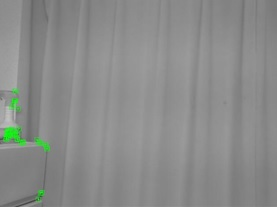
\includegraphics[width=1.0\linewidth]{figs/Tracking02.jpg}
        \caption{図\ref{fig:picture02}赤線部のカメラ画像}
        \label{fig:Tracking02}
  \end{minipage}

 \end{tabular}
\end{figure}

ここでトラッキングを継続させるためにマーカを使用する。本実験では直径19.5[mm]のシールをマーカとして使用する。

\begin{figure}[h]
        \begin{center}
        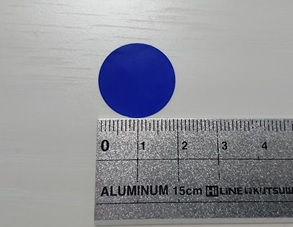
\includegraphics[width=0.6\linewidth]{figs/marker01.jpg}
        \caption{マーカとして使用するシール}
        \label{fig:marker01}
        \end{center}
\end{figure}

\newpage

トラッキング継続に必要なマーカを絞り込むため、以下に示す手順を行う。


\begin{enumerate}
   \item カメラからの距離1[m],高さ1[m]地点のカーテン表面を中心にマーカを貼り付ける。
   \item マーカのみをトラッキングするようにカメラをカーテン方向へ回転する。
   \item マーカを100[mm]間隔で縦方向に増やす。SLAMを再起動し再び手順2を行う。これをトラッキング可能になるまで繰り返す。
  \item マーカの間隔を10[mm]狭める。SLAMを再起動し再び手順2を行う。これをトラッキング不能になるまで繰り返す。
  \item マーカの間隔を1[mm]広げてSLAMを再起動し2を行う。これをトラッキング可能になるまで繰り返す。
   \item マーカの間隔と特徴点マッチング数を記録する。
\end{enumerate}

\begin{figure}[h]
        \begin{center}
        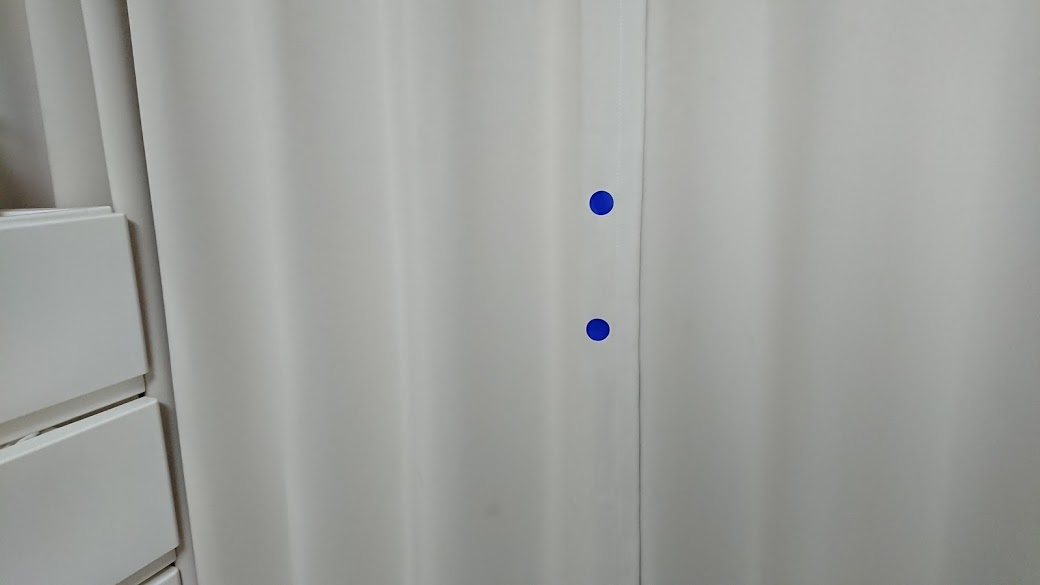
\includegraphics[width=0.7\linewidth]{figs/marker03.jpg}
        \caption{カーテン表面に貼付されたマーカ}
        \label{fig:marker03}
        \end{center}
\end{figure}

\newpage

\section{実験結果}

シール1〜3枚をマーカとしたときはトラッキング不能であった。シール4枚をマーカとした時に特徴点マッチング数95〜121を獲得しトラッキング継続に成功した。間隔は47[mm]までは安定していたが,46[mm]になると特徴点の消失と復帰を繰り返す不安定な動作となった。以上より、本実験では47[mm]間隔で配置された4枚のシールが単眼カメラSLAMを完遂できる最小範囲のマーカとなった。

\begin{figure}[h]
        \begin{center}
        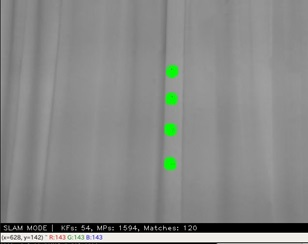
\includegraphics[width=0.7\linewidth]{figs/Tracking03.jpg}
        \caption{マーカのみでトラッキング継続成功}
        \label{fig:Tracking03}
        \end{center}
\end{figure}

